\documentclass[1p]{elsarticle_modified}
%\bibliographystyle{elsarticle-num}

%\usepackage[colorlinks]{hyperref}
%\usepackage{abbrmath_seonhwa} %\Abb, \Ascr, \Acal ,\Abf, \Afrak
\usepackage{amsfonts}
\usepackage{amssymb}
\usepackage{amsmath}
\usepackage{amsthm}
\usepackage{scalefnt}
\usepackage{amsbsy}
\usepackage{kotex}
\usepackage{caption}
\usepackage{subfig}
\usepackage{color}
\usepackage{graphicx}
\usepackage{xcolor} %% white, black, red, green, blue, cyan, magenta, yellow
\usepackage{float}
\usepackage{setspace}
\usepackage{hyperref}

\usepackage{tikz}
\usetikzlibrary{arrows}

\usepackage{multirow}
\usepackage{array} % fixed length table
\usepackage{hhline}

%%%%%%%%%%%%%%%%%%%%%
\makeatletter
\renewcommand*\env@matrix[1][\arraystretch]{%
	\edef\arraystretch{#1}%
	\hskip -\arraycolsep
	\let\@ifnextchar\new@ifnextchar
	\array{*\c@MaxMatrixCols c}}
\makeatother %https://tex.stackexchange.com/questions/14071/how-can-i-increase-the-line-spacing-in-a-matrix
%%%%%%%%%%%%%%%

\usepackage[normalem]{ulem}

\newcommand{\msout}[1]{\ifmmode\text{\sout{\ensuremath{#1}}}\else\sout{#1}\fi}
%SOURCE: \msout is \stkout macro in https://tex.stackexchange.com/questions/20609/strikeout-in-math-mode

\newcommand{\cancel}[1]{
	\ifmmode
	{\color{red}\msout{#1}}
	\else
	{\color{red}\sout{#1}}
	\fi
}

\newcommand{\add}[1]{
	{\color{blue}\uwave{#1}}
}

\newcommand{\replace}[2]{
	\ifmmode
	{\color{red}\msout{#1}}{\color{blue}\uwave{#2}}
	\else
	{\color{red}\sout{#1}}{\color{blue}\uwave{#2}}
	\fi
}

\newcommand{\Sol}{\mathcal{S}} %segment
\newcommand{\D}{D} %diagram
\newcommand{\A}{\mathcal{A}} %arc


%%%%%%%%%%%%%%%%%%%%%%%%%%%%%5 test

\def\sl{\operatorname{\textup{SL}}(2,\Cbb)}
\def\psl{\operatorname{\textup{PSL}}(2,\Cbb)}
\def\quan{\mkern 1mu \triangleright \mkern 1mu}

\theoremstyle{definition}
\newtheorem{thm}{Theorem}[section]
\newtheorem{prop}[thm]{Proposition}
\newtheorem{lem}[thm]{Lemma}
\newtheorem{ques}[thm]{Question}
\newtheorem{cor}[thm]{Corollary}
\newtheorem{defn}[thm]{Definition}
\newtheorem{exam}[thm]{Example}
\newtheorem{rmk}[thm]{Remark}
\newtheorem{alg}[thm]{Algorithm}

\newcommand{\I}{\sqrt{-1}}
\begin{document}

%\begin{frontmatter}
%
%\title{Boundary parabolic representations of knots up to 8 crossings}
%
%%% Group authors per affiliation:
%\author{Yunhi Cho} 
%\address{Department of Mathematics, University of Seoul, Seoul, Korea}
%\ead{yhcho@uos.ac.kr}
%
%
%\author{Seonhwa Kim} %\fnref{s_kim}}
%\address{Center for Geometry and Physics, Institute for Basic Science, Pohang, 37673, Korea}
%\ead{ryeona17@ibs.re.kr}
%
%\author{Hyuk Kim}
%\address{Department of Mathematical Sciences, Seoul National University, Seoul 08826, Korea}
%\ead{hyukkim@snu.ac.kr}
%
%\author{Seokbeom Yoon}
%\address{Department of Mathematical Sciences, Seoul National University, Seoul, 08826,  Korea}
%\ead{sbyoon15@snu.ac.kr}
%
%\begin{abstract}
%We find all boundary parabolic representation of knots up to 8 crossings.
%
%\end{abstract}
%\begin{keyword}
%    \MSC[2010] 57M25 
%\end{keyword}
%
%\end{frontmatter}

%\linenumbers
%\tableofcontents
%
\newcommand\colored[1]{\textcolor{white}{\rule[-0.35ex]{0.8em}{1.4ex}}\kern-0.8em\color{red} #1}%
%\newcommand\colored[1]{\textcolor{white}{ #1}\kern-2.17ex	\textcolor{white}{ #1}\kern-1.81ex	\textcolor{white}{ #1}\kern-2.15ex\color{red}#1	}

{\Large $\underline{12n_{0263}~(K12n_{0263})}$}

\setlength{\tabcolsep}{10pt}
\renewcommand{\arraystretch}{1.6}
\vspace{1cm}\begin{tabular}{m{100pt}>{\centering\arraybackslash}m{274pt}}
\multirow{5}{120pt}{
	\centering
	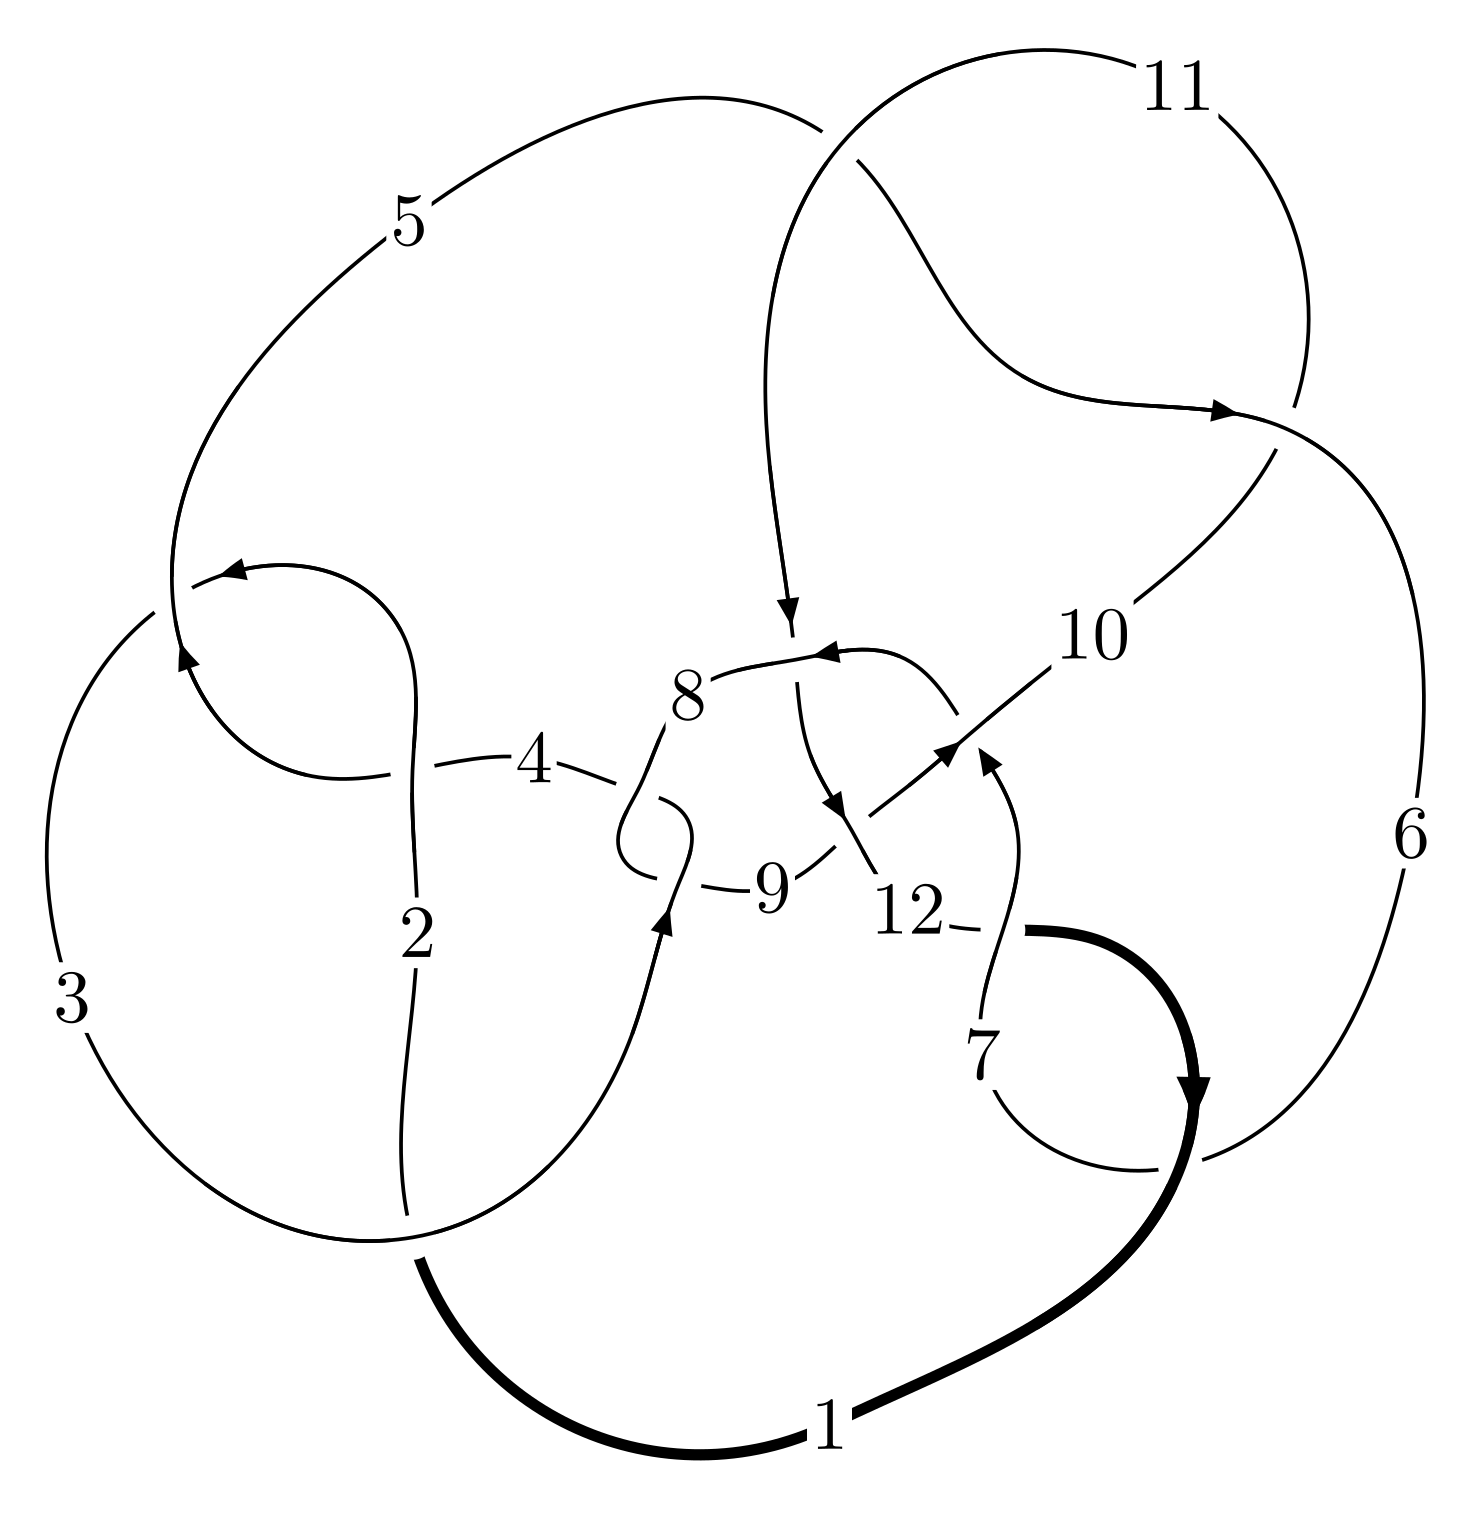
\includegraphics[width=112pt]{../../../GIT/diagram.site/Diagrams/png/2352_12n_0263.png}\\
\ \ \ A knot diagram\footnotemark}&
\allowdisplaybreaks
\textbf{Linearized knot diagam} \\
\cline{2-2}
 &
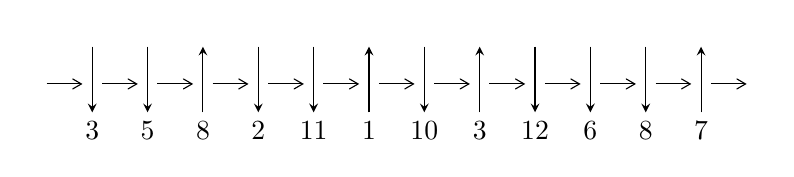
\begin{tikzpicture}[x=20pt, y=17pt]
	% nodes
	\node (C0) at (0, 0) {};
	\node (C1) at (1, 0) {};
	\node (C1U) at (1, +1) {};
	\node (C1D) at (1, -1) {3};

	\node (C2) at (2, 0) {};
	\node (C2U) at (2, +1) {};
	\node (C2D) at (2, -1) {5};

	\node (C3) at (3, 0) {};
	\node (C3U) at (3, +1) {};
	\node (C3D) at (3, -1) {8};

	\node (C4) at (4, 0) {};
	\node (C4U) at (4, +1) {};
	\node (C4D) at (4, -1) {2};

	\node (C5) at (5, 0) {};
	\node (C5U) at (5, +1) {};
	\node (C5D) at (5, -1) {11};

	\node (C6) at (6, 0) {};
	\node (C6U) at (6, +1) {};
	\node (C6D) at (6, -1) {1};

	\node (C7) at (7, 0) {};
	\node (C7U) at (7, +1) {};
	\node (C7D) at (7, -1) {10};

	\node (C8) at (8, 0) {};
	\node (C8U) at (8, +1) {};
	\node (C8D) at (8, -1) {3};

	\node (C9) at (9, 0) {};
	\node (C9U) at (9, +1) {};
	\node (C9D) at (9, -1) {12};

	\node (C10) at (10, 0) {};
	\node (C10U) at (10, +1) {};
	\node (C10D) at (10, -1) {6};

	\node (C11) at (11, 0) {};
	\node (C11U) at (11, +1) {};
	\node (C11D) at (11, -1) {8};

	\node (C12) at (12, 0) {};
	\node (C12U) at (12, +1) {};
	\node (C12D) at (12, -1) {7};
	\node (C13) at (13, 0) {};

	% arrows
	\draw[->,>={angle 60}]
	(C0) edge (C1) (C1) edge (C2) (C2) edge (C3) (C3) edge (C4) (C4) edge (C5) (C5) edge (C6) (C6) edge (C7) (C7) edge (C8) (C8) edge (C9) (C9) edge (C10) (C10) edge (C11) (C11) edge (C12) (C12) edge (C13) ;	\draw[->,>=stealth]
	(C1U) edge (C1D) (C2U) edge (C2D) (C3D) edge (C3U) (C4U) edge (C4D) (C5U) edge (C5D) (C6D) edge (C6U) (C7U) edge (C7D) (C8D) edge (C8U) (C9U) edge (C9D) (C10U) edge (C10D) (C11U) edge (C11D) (C12D) edge (C12U) ;
	\end{tikzpicture} \\
\hhline{~~} \\& 
\textbf{Solving Sequence} \\ \cline{2-2} 
 &
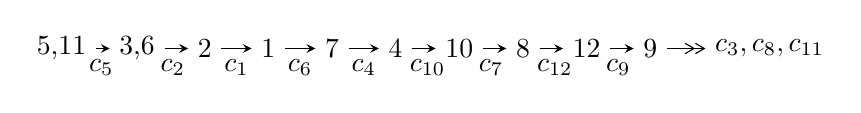
\begin{tikzpicture}[x=23pt, y=7pt]
	% node
	\node (A0) at (-1/8, 0) {5,11};
	\node (A1) at (17/16, 0) {3,6};
	\node (A2) at (17/8, 0) {2};
	\node (A3) at (25/8, 0) {1};
	\node (A4) at (33/8, 0) {7};
	\node (A5) at (41/8, 0) {4};
	\node (A6) at (49/8, 0) {10};
	\node (A7) at (57/8, 0) {8};
	\node (A8) at (65/8, 0) {12};
	\node (A9) at (73/8, 0) {9};
	\node (C1) at (1/2, -1) {$c_{5}$};
	\node (C2) at (13/8, -1) {$c_{2}$};
	\node (C3) at (21/8, -1) {$c_{1}$};
	\node (C4) at (29/8, -1) {$c_{6}$};
	\node (C5) at (37/8, -1) {$c_{4}$};
	\node (C6) at (45/8, -1) {$c_{10}$};
	\node (C7) at (53/8, -1) {$c_{7}$};
	\node (C8) at (61/8, -1) {$c_{12}$};
	\node (C9) at (69/8, -1) {$c_{9}$};
	\node (A10) at (11, 0) {$c_{3},c_{8},c_{11}$};

	% edge
	\draw[->,>=stealth]	
	(A0) edge (A1) (A1) edge (A2) (A2) edge (A3) (A3) edge (A4) (A4) edge (A5) (A5) edge (A6) (A6) edge (A7) (A7) edge (A8) (A8) edge (A9) ;
	\draw[->>,>={angle 60}]	
	(A9) edge (A10);
\end{tikzpicture} \\ 

\end{tabular} \\

\footnotetext{
The image of knot diagram is generated by the software ``\textbf{Draw programme}" developed by Andrew Bartholomew(\url{http://www.layer8.co.uk/maths/draw/index.htm\#Running-draw}), where we modified some parts for our purpose(\url{https://github.com/CATsTAILs/LinksPainter}).
}\phantom \\ \newline 
\centering \textbf{Ideals for irreducible components\footnotemark of $X_{\text{par}}$} 
 
\begin{align*}
I^u_{1}&=\langle 
-5.10710\times10^{324} u^{87}-9.56312\times10^{325} u^{86}+\cdots+1.34371\times10^{329} b+2.04185\times10^{329},\\
\phantom{I^u_{1}}&\phantom{= \langle  }1.04950\times10^{330} u^{87}+1.94168\times10^{330} u^{86}+\cdots+2.37970\times10^{332} a-5.85379\times10^{332},\\
\phantom{I^u_{1}}&\phantom{= \langle  }u^{88}+2 u^{87}+\cdots+4968 u-1771\rangle \\
I^u_{2}&=\langle 
b+1,\;6 u^8+7 u^7+12 u^6+8 u^5+17 u^4+10 u^3+9 u^2+7 a+5 u+8,\\
\phantom{I^u_{2}}&\phantom{= \langle  }u^9+u^8+2 u^7+u^6+3 u^5+u^4+2 u^3+u-1\rangle \\
I^u_{3}&=\langle 
2 u^{15}-2 u^{14}+\cdots+b-2,\;3 u^{15}- u^{14}+\cdots+a+5 u,\;u^{16}+8 u^{14}+\cdots+3 u+1\rangle \\
\\
\end{align*}
\raggedright * 3 irreducible components of $\dim_{\mathbb{C}}=0$, with total 113 representations.\\
\footnotetext{All coefficients of polynomials are rational numbers. But the coefficients are sometimes approximated in decimal forms when there is not enough margin.}
\newpage
\renewcommand{\arraystretch}{1}
\centering \section*{I. $I^u_{1}= \langle -5.11\times10^{324} u^{87}-9.56\times10^{325} u^{86}+\cdots+1.34\times10^{329} b+2.04\times10^{329},\;1.05\times10^{330} u^{87}+1.94\times10^{330} u^{86}+\cdots+2.38\times10^{332} a-5.85\times10^{332},\;u^{88}+2 u^{87}+\cdots+4968 u-1771 \rangle$}
\flushleft \textbf{(i) Arc colorings}\\
\begin{tabular}{m{7pt} m{180pt} m{7pt} m{180pt} }
\flushright $a_{5}=$&$\begin{pmatrix}1\\0\end{pmatrix}$ \\
\flushright $a_{11}=$&$\begin{pmatrix}0\\u\end{pmatrix}$ \\
\flushright $a_{3}=$&$\begin{pmatrix}-0.00441021 u^{87}-0.00815934 u^{86}+\cdots+21.8561 u+2.45988\\0.0000380076 u^{87}+0.000711697 u^{86}+\cdots+9.10028 u-1.51957\end{pmatrix}$ \\
\flushright $a_{6}=$&$\begin{pmatrix}1\\u^2\end{pmatrix}$ \\
\flushright $a_{2}=$&$\begin{pmatrix}-0.00437220 u^{87}-0.00744764 u^{86}+\cdots+30.9564 u+0.940316\\0.0000380076 u^{87}+0.000711697 u^{86}+\cdots+9.10028 u-1.51957\end{pmatrix}$ \\
\flushright $a_{1}=$&$\begin{pmatrix}-0.00153178 u^{87}-0.00266896 u^{86}+\cdots+23.2890 u-2.25667\\-0.000996652 u^{87}-0.00124794 u^{86}+\cdots+14.3592 u-2.12843\end{pmatrix}$ \\
\flushright $a_{7}=$&$\begin{pmatrix}-0.00142383 u^{87}-0.00605369 u^{86}+\cdots-33.0919 u+13.1203\\-0.000364423 u^{87}-0.00102860 u^{86}+\cdots-28.1927 u+9.11040\end{pmatrix}$ \\
\flushright $a_{4}=$&$\begin{pmatrix}-0.00292538 u^{87}-0.00347282 u^{86}+\cdots+53.4302 u-13.5553\\-0.000932894 u^{87}+0.0000161336 u^{86}+\cdots+34.8142 u-9.59675\end{pmatrix}$ \\
\flushright $a_{10}=$&$\begin{pmatrix}u\\u^3+u\end{pmatrix}$ \\
\flushright $a_{8}=$&$\begin{pmatrix}-0.00119455 u^{87}-0.00482926 u^{86}+\cdots-31.9654 u+12.3640\\-0.000562133 u^{87}-0.00184393 u^{86}+\cdots-30.4650 u+9.71045\end{pmatrix}$ \\
\flushright $a_{12}=$&$\begin{pmatrix}0.00596932 u^{87}+0.0100899 u^{86}+\cdots-21.3404 u-4.51265\\0.00269198 u^{87}+0.00756739 u^{86}+\cdots+12.7020 u-10.9619\end{pmatrix}$ \\
\flushright $a_{9}=$&$\begin{pmatrix}0.00392308 u^{87}+0.00976005 u^{86}+\cdots-4.05932 u-10.1331\\0.00259711 u^{87}+0.00552722 u^{86}+\cdots+16.4800 u-8.72611\end{pmatrix}$\\&\end{tabular}
\flushleft \textbf{(ii) Obstruction class $= -1$}\\~\\
\flushleft \textbf{(iii) Cusp Shapes $= -0.0135860 u^{87}-0.0234158 u^{86}+\cdots+148.906 u-31.3158$}\\~\\
\newpage\renewcommand{\arraystretch}{1}
\flushleft \textbf{(iv) u-Polynomials at the component}\newline \\
\begin{tabular}{m{50pt}|m{274pt}}
Crossings & \hspace{64pt}u-Polynomials at each crossing \\
\hline $$\begin{aligned}c_{1}\end{aligned}$$&$\begin{aligned}
&u^{88}+36 u^{87}+\cdots+9016 u+2401
\end{aligned}$\\
\hline $$\begin{aligned}c_{2},c_{4}\end{aligned}$$&$\begin{aligned}
&u^{88}-16 u^{87}+\cdots+504 u-49
\end{aligned}$\\
\hline $$\begin{aligned}c_{3},c_{8}\end{aligned}$$&$\begin{aligned}
&u^{88}+u^{87}+\cdots+14336 u+25088
\end{aligned}$\\
\hline $$\begin{aligned}c_{5},c_{10}\end{aligned}$$&$\begin{aligned}
&u^{88}+2 u^{87}+\cdots+4968 u-1771
\end{aligned}$\\
\hline $$\begin{aligned}c_{6},c_{12}\end{aligned}$$&$\begin{aligned}
&u^{88}+3 u^{87}+\cdots-1497 u-181
\end{aligned}$\\
\hline $$\begin{aligned}c_{7}\end{aligned}$$&$\begin{aligned}
&u^{88}-4 u^{87}+\cdots+2 u-1
\end{aligned}$\\
\hline $$\begin{aligned}c_{9}\end{aligned}$$&$\begin{aligned}
&u^{88}-14 u^{87}+\cdots-5848 u+1043
\end{aligned}$\\
\hline $$\begin{aligned}c_{11}\end{aligned}$$&$\begin{aligned}
&u^{88}- u^{87}+\cdots+8558243 u-2435537
\end{aligned}$\\
\hline
\end{tabular}\\~\\
\newpage\renewcommand{\arraystretch}{1}
\flushleft \textbf{(v) Riley Polynomials at the component}\newline \\
\begin{tabular}{m{50pt}|m{274pt}}
Crossings & \hspace{64pt}Riley Polynomials at each crossing \\
\hline $$\begin{aligned}c_{1}\end{aligned}$$&$\begin{aligned}
&y^{88}+48 y^{87}+\cdots-1539089020 y+5764801
\end{aligned}$\\
\hline $$\begin{aligned}c_{2},c_{4}\end{aligned}$$&$\begin{aligned}
&y^{88}-36 y^{87}+\cdots-9016 y+2401
\end{aligned}$\\
\hline $$\begin{aligned}c_{3},c_{8}\end{aligned}$$&$\begin{aligned}
&y^{88}-63 y^{87}+\cdots-10096214016 y+629407744
\end{aligned}$\\
\hline $$\begin{aligned}c_{5},c_{10}\end{aligned}$$&$\begin{aligned}
&y^{88}+70 y^{87}+\cdots+39623986 y+3136441
\end{aligned}$\\
\hline $$\begin{aligned}c_{6},c_{12}\end{aligned}$$&$\begin{aligned}
&y^{88}+49 y^{87}+\cdots-883509 y+32761
\end{aligned}$\\
\hline $$\begin{aligned}c_{7}\end{aligned}$$&$\begin{aligned}
&y^{88}-16 y^{87}+\cdots+6 y+1
\end{aligned}$\\
\hline $$\begin{aligned}c_{9}\end{aligned}$$&$\begin{aligned}
&y^{88}+2 y^{87}+\cdots+12594048 y+1087849
\end{aligned}$\\
\hline $$\begin{aligned}c_{11}\end{aligned}$$&$\begin{aligned}
&y^{88}+33 y^{87}+\cdots+85934090519941 y+5931840478369
\end{aligned}$\\
\hline
\end{tabular}\\~\\
\newpage\flushleft \textbf{(vi) Complex Volumes and Cusp Shapes}
$$\begin{array}{c|c|c}  
\text{Solutions to }I^u_{1}& \I (\text{vol} + \sqrt{-1}CS) & \text{Cusp shape}\\
 \hline 
\begin{aligned}
u &= -0.805310 + 0.589984 I \\
a &= \phantom{-}0.939329 + 0.447844 I \\
b &= \phantom{-}1.000810 - 0.612397 I\end{aligned}
 & -0.95191 + 5.34222 I & \phantom{-0.000000 } 0 \\ \hline\begin{aligned}
u &= -0.805310 - 0.589984 I \\
a &= \phantom{-}0.939329 - 0.447844 I \\
b &= \phantom{-}1.000810 + 0.612397 I\end{aligned}
 & -0.95191 - 5.34222 I & \phantom{-0.000000 } 0 \\ \hline\begin{aligned}
u &= \phantom{-}0.992163 + 0.083390 I \\
a &= \phantom{-}0.306400 + 0.290281 I \\
b &= -0.860253 - 0.469883 I\end{aligned}
 & -3.57000 - 4.86222 I & \phantom{-0.000000 } 0 \\ \hline\begin{aligned}
u &= \phantom{-}0.992163 - 0.083390 I \\
a &= \phantom{-}0.306400 - 0.290281 I \\
b &= -0.860253 + 0.469883 I\end{aligned}
 & -3.57000 + 4.86222 I & \phantom{-0.000000 } 0 \\ \hline\begin{aligned}
u &= \phantom{-}0.948677 + 0.240901 I \\
a &= \phantom{-}0.257262 + 0.041899 I \\
b &= \phantom{-}0.816492 - 0.831232 I\end{aligned}
 & \phantom{-}4.48132 + 0.68778 I & \phantom{-0.000000 } 0 \\ \hline\begin{aligned}
u &= \phantom{-}0.948677 - 0.240901 I \\
a &= \phantom{-}0.257262 - 0.041899 I \\
b &= \phantom{-}0.816492 + 0.831232 I\end{aligned}
 & \phantom{-}4.48132 - 0.68778 I & \phantom{-0.000000 } 0 \\ \hline\begin{aligned}
u &= \phantom{-}0.139706 + 0.952235 I \\
a &= -0.925127 + 0.095450 I \\
b &= \phantom{-}1.61154 - 0.00181 I\end{aligned}
 & -8.88186 - 0.52240 I & \phantom{-0.000000 } 0 \\ \hline\begin{aligned}
u &= \phantom{-}0.139706 - 0.952235 I \\
a &= -0.925127 - 0.095450 I \\
b &= \phantom{-}1.61154 + 0.00181 I\end{aligned}
 & -8.88186 + 0.52240 I & \phantom{-0.000000 } 0 \\ \hline\begin{aligned}
u &= \phantom{-}0.517483 + 0.776305 I \\
a &= -1.78011 + 2.41840 I \\
b &= -0.936656 + 0.081694 I\end{aligned}
 & -2.86090 - 2.57918 I & \phantom{-0.000000 } 0 \\ \hline\begin{aligned}
u &= \phantom{-}0.517483 - 0.776305 I \\
a &= -1.78011 - 2.41840 I \\
b &= -0.936656 - 0.081694 I\end{aligned}
 & -2.86090 + 2.57918 I & \phantom{-0.000000 } 0\\
 \hline 
 \end{array}$$\newpage$$\begin{array}{c|c|c}  
\text{Solutions to }I^u_{1}& \I (\text{vol} + \sqrt{-1}CS) & \text{Cusp shape}\\
 \hline 
\begin{aligned}
u &= \phantom{-}0.919116 + 0.059965 I \\
a &= \phantom{-}0.926180 + 0.256722 I \\
b &= \phantom{-}0.955514 - 0.798995 I\end{aligned}
 & \phantom{-}4.06052 + 5.39830 I & \phantom{-0.000000 } 0 \\ \hline\begin{aligned}
u &= \phantom{-}0.919116 - 0.059965 I \\
a &= \phantom{-}0.926180 - 0.256722 I \\
b &= \phantom{-}0.955514 + 0.798995 I\end{aligned}
 & \phantom{-}4.06052 - 5.39830 I & \phantom{-0.000000 } 0 \\ \hline\begin{aligned}
u &= -0.740792 + 0.830928 I \\
a &= \phantom{-}0.971335 + 0.053984 I \\
b &= \phantom{-}0.063149 - 0.256272 I\end{aligned}
 & -0.52740 + 2.78156 I & \phantom{-0.000000 } 0 \\ \hline\begin{aligned}
u &= -0.740792 - 0.830928 I \\
a &= \phantom{-}0.971335 - 0.053984 I \\
b &= \phantom{-}0.063149 + 0.256272 I\end{aligned}
 & -0.52740 - 2.78156 I & \phantom{-0.000000 } 0 \\ \hline\begin{aligned}
u &= -0.248018 + 0.848575 I \\
a &= \phantom{-}4.78654 - 1.31097 I \\
b &= -0.711645 + 0.146889 I\end{aligned}
 & -2.35191 + 3.21223 I & -7.96555 - 6.35540 I \\ \hline\begin{aligned}
u &= -0.248018 - 0.848575 I \\
a &= \phantom{-}4.78654 + 1.31097 I \\
b &= -0.711645 - 0.146889 I\end{aligned}
 & -2.35191 - 3.21223 I & -7.96555 + 6.35540 I \\ \hline\begin{aligned}
u &= -0.079212 + 1.132010 I \\
a &= -0.24213 + 2.07975 I \\
b &= \phantom{-}0.808393 - 0.790949 I\end{aligned}
 & \phantom{-}2.28913 - 1.10084 I & \phantom{-0.000000 } 0 \\ \hline\begin{aligned}
u &= -0.079212 - 1.132010 I \\
a &= -0.24213 - 2.07975 I \\
b &= \phantom{-}0.808393 + 0.790949 I\end{aligned}
 & \phantom{-}2.28913 + 1.10084 I & \phantom{-0.000000 } 0 \\ \hline\begin{aligned}
u &= \phantom{-}0.319029 + 1.102470 I \\
a &= \phantom{-}0.16501 - 1.71908 I \\
b &= \phantom{-}1.18756 + 0.90857 I\end{aligned}
 & \phantom{-}6.66068 - 5.31014 I & \phantom{-0.000000 } 0 \\ \hline\begin{aligned}
u &= \phantom{-}0.319029 - 1.102470 I \\
a &= \phantom{-}0.16501 + 1.71908 I \\
b &= \phantom{-}1.18756 - 0.90857 I\end{aligned}
 & \phantom{-}6.66068 + 5.31014 I & \phantom{-0.000000 } 0\\
 \hline 
 \end{array}$$\newpage$$\begin{array}{c|c|c}  
\text{Solutions to }I^u_{1}& \I (\text{vol} + \sqrt{-1}CS) & \text{Cusp shape}\\
 \hline 
\begin{aligned}
u &= -0.174859 + 0.815548 I \\
a &= \phantom{-}0.677317 + 0.300319 I \\
b &= \phantom{-}0.575930 + 0.151275 I\end{aligned}
 & \phantom{-}1.08551 + 1.92358 I & \phantom{-}4.64840 - 3.23156 I \\ \hline\begin{aligned}
u &= -0.174859 - 0.815548 I \\
a &= \phantom{-}0.677317 - 0.300319 I \\
b &= \phantom{-}0.575930 - 0.151275 I\end{aligned}
 & \phantom{-}1.08551 - 1.92358 I & \phantom{-}4.64840 + 3.23156 I \\ \hline\begin{aligned}
u &= -0.767240 + 0.896651 I \\
a &= \phantom{-}0.121871 + 0.271621 I \\
b &= \phantom{-}0.760360 + 0.637175 I\end{aligned}
 & -0.156171 + 0.447897 I & \phantom{-0.000000 } 0 \\ \hline\begin{aligned}
u &= -0.767240 - 0.896651 I \\
a &= \phantom{-}0.121871 - 0.271621 I \\
b &= \phantom{-}0.760360 - 0.637175 I\end{aligned}
 & -0.156171 - 0.447897 I & \phantom{-0.000000 } 0 \\ \hline\begin{aligned}
u &= \phantom{-}0.237078 + 0.779145 I \\
a &= -1.16266 + 0.85834 I \\
b &= -1.135060 - 0.295927 I\end{aligned}
 & -2.63864 - 1.15581 I & -8.11133 + 0. I\phantom{ +0.000000I} \\ \hline\begin{aligned}
u &= \phantom{-}0.237078 - 0.779145 I \\
a &= -1.16266 - 0.85834 I \\
b &= -1.135060 + 0.295927 I\end{aligned}
 & -2.63864 + 1.15581 I & -8.11133 + 0. I\phantom{ +0.000000I} \\ \hline\begin{aligned}
u &= -0.451795 + 1.101000 I \\
a &= \phantom{-}0.528741 - 0.757913 I \\
b &= -0.311022 + 0.556483 I\end{aligned}
 & \phantom{-}0.22772 + 2.36626 I & \phantom{-0.000000 } 0 \\ \hline\begin{aligned}
u &= -0.451795 - 1.101000 I \\
a &= \phantom{-}0.528741 + 0.757913 I \\
b &= -0.311022 - 0.556483 I\end{aligned}
 & \phantom{-}0.22772 - 2.36626 I & \phantom{-0.000000 } 0 \\ \hline\begin{aligned}
u &= \phantom{-}0.938892 + 0.789370 I \\
a &= \phantom{-}0.381760 - 0.534102 I \\
b &= \phantom{-}0.744153 + 0.149516 I\end{aligned}
 & -5.45148 + 0.98119 I & \phantom{-0.000000 } 0 \\ \hline\begin{aligned}
u &= \phantom{-}0.938892 - 0.789370 I \\
a &= \phantom{-}0.381760 + 0.534102 I \\
b &= \phantom{-}0.744153 - 0.149516 I\end{aligned}
 & -5.45148 - 0.98119 I & \phantom{-0.000000 } 0\\
 \hline 
 \end{array}$$\newpage$$\begin{array}{c|c|c}  
\text{Solutions to }I^u_{1}& \I (\text{vol} + \sqrt{-1}CS) & \text{Cusp shape}\\
 \hline 
\begin{aligned}
u &= \phantom{-}0.785869 + 0.950757 I \\
a &= \phantom{-}0.384303 - 0.295118 I \\
b &= \phantom{-}0.839629 + 0.078942 I\end{aligned}
 & -4.90136 - 7.25149 I & \phantom{-0.000000 } 0 \\ \hline\begin{aligned}
u &= \phantom{-}0.785869 - 0.950757 I \\
a &= \phantom{-}0.384303 + 0.295118 I \\
b &= \phantom{-}0.839629 - 0.078942 I\end{aligned}
 & -4.90136 + 7.25149 I & \phantom{-0.000000 } 0 \\ \hline\begin{aligned}
u &= \phantom{-}0.135066 + 1.254400 I \\
a &= -0.86601 - 1.61832 I \\
b &= \phantom{-}0.951322 + 0.752407 I\end{aligned}
 & \phantom{-}1.84545 - 6.92325 I & \phantom{-0.000000 } 0 \\ \hline\begin{aligned}
u &= \phantom{-}0.135066 - 1.254400 I \\
a &= -0.86601 + 1.61832 I \\
b &= \phantom{-}0.951322 - 0.752407 I\end{aligned}
 & \phantom{-}1.84545 + 6.92325 I & \phantom{-0.000000 } 0 \\ \hline\begin{aligned}
u &= \phantom{-}0.166697 + 1.254150 I \\
a &= \phantom{-}0.45531 - 1.38825 I \\
b &= -0.879422 + 0.969350 I\end{aligned}
 & \phantom{-}1.34449 - 3.11057 I & \phantom{-0.000000 } 0 \\ \hline\begin{aligned}
u &= \phantom{-}0.166697 - 1.254150 I \\
a &= \phantom{-}0.45531 + 1.38825 I \\
b &= -0.879422 - 0.969350 I\end{aligned}
 & \phantom{-}1.34449 + 3.11057 I & \phantom{-0.000000 } 0 \\ \hline\begin{aligned}
u &= \phantom{-}0.128440 + 1.272930 I \\
a &= -0.271149 + 0.753744 I \\
b &= -1.331880 - 0.096691 I\end{aligned}
 & \phantom{-}1.74481 - 1.77274 I & \phantom{-0.000000 } 0 \\ \hline\begin{aligned}
u &= \phantom{-}0.128440 - 1.272930 I \\
a &= -0.271149 - 0.753744 I \\
b &= -1.331880 + 0.096691 I\end{aligned}
 & \phantom{-}1.74481 + 1.77274 I & \phantom{-0.000000 } 0 \\ \hline\begin{aligned}
u &= -0.696650 + 0.064826 I \\
a &= -0.85984 - 3.03345 I \\
b &= -1.216760 + 0.127728 I\end{aligned}
 & -4.59376 - 2.75184 I & -8.12364 + 4.75878 I \\ \hline\begin{aligned}
u &= -0.696650 - 0.064826 I \\
a &= -0.85984 + 3.03345 I \\
b &= -1.216760 - 0.127728 I\end{aligned}
 & -4.59376 + 2.75184 I & -8.12364 - 4.75878 I\\
 \hline 
 \end{array}$$\newpage$$\begin{array}{c|c|c}  
\text{Solutions to }I^u_{1}& \I (\text{vol} + \sqrt{-1}CS) & \text{Cusp shape}\\
 \hline 
\begin{aligned}
u &= \phantom{-}0.112427 + 1.300630 I \\
a &= -0.610156 + 1.055710 I \\
b &= \phantom{-}0.671732 - 1.206590 I\end{aligned}
 & \phantom{-}8.28391 + 2.17535 I & \phantom{-0.000000 } 0 \\ \hline\begin{aligned}
u &= \phantom{-}0.112427 - 1.300630 I \\
a &= -0.610156 - 1.055710 I \\
b &= \phantom{-}0.671732 + 1.206590 I\end{aligned}
 & \phantom{-}8.28391 - 2.17535 I & \phantom{-0.000000 } 0 \\ \hline\begin{aligned}
u &= -0.313929 + 1.278860 I \\
a &= \phantom{-}0.149566 - 0.089877 I \\
b &= -1.57140 - 0.02860 I\end{aligned}
 & -0.73301 + 6.46230 I & \phantom{-0.000000 } 0 \\ \hline\begin{aligned}
u &= -0.313929 - 1.278860 I \\
a &= \phantom{-}0.149566 + 0.089877 I \\
b &= -1.57140 + 0.02860 I\end{aligned}
 & -0.73301 - 6.46230 I & \phantom{-0.000000 } 0 \\ \hline\begin{aligned}
u &= -0.266726 + 1.305550 I \\
a &= \phantom{-}0.20459 - 1.68443 I \\
b &= -0.771564 + 0.690828 I\end{aligned}
 & \phantom{-}3.68905 + 4.17717 I & \phantom{-0.000000 } 0 \\ \hline\begin{aligned}
u &= -0.266726 - 1.305550 I \\
a &= \phantom{-}0.20459 + 1.68443 I \\
b &= -0.771564 - 0.690828 I\end{aligned}
 & \phantom{-}3.68905 - 4.17717 I & \phantom{-0.000000 } 0 \\ \hline\begin{aligned}
u &= -0.021756 + 1.350550 I \\
a &= \phantom{-}0.54100 + 1.31164 I \\
b &= -1.064570 - 0.638718 I\end{aligned}
 & \phantom{-}2.82569 - 0.98099 I & \phantom{-0.000000 } 0 \\ \hline\begin{aligned}
u &= -0.021756 - 1.350550 I \\
a &= \phantom{-}0.54100 - 1.31164 I \\
b &= -1.064570 + 0.638718 I\end{aligned}
 & \phantom{-}2.82569 + 0.98099 I & \phantom{-0.000000 } 0 \\ \hline\begin{aligned}
u &= \phantom{-}0.018865 + 0.638570 I \\
a &= \phantom{-}0.311943 + 0.067730 I \\
b &= \phantom{-}0.240022 + 0.542471 I\end{aligned}
 & \phantom{-}0.93570 + 1.73737 I & \phantom{-}2.01048 - 1.71572 I \\ \hline\begin{aligned}
u &= \phantom{-}0.018865 - 0.638570 I \\
a &= \phantom{-}0.311943 - 0.067730 I \\
b &= \phantom{-}0.240022 - 0.542471 I\end{aligned}
 & \phantom{-}0.93570 - 1.73737 I & \phantom{-}2.01048 + 1.71572 I\\
 \hline 
 \end{array}$$\newpage$$\begin{array}{c|c|c}  
\text{Solutions to }I^u_{1}& \I (\text{vol} + \sqrt{-1}CS) & \text{Cusp shape}\\
 \hline 
\begin{aligned}
u &= -0.588985\phantom{ +0.000000I} \\
a &= \phantom{-}1.28655\phantom{ +0.000000I} \\
b &= \phantom{-}0.415532\phantom{ +0.000000I}\end{aligned}
 & -1.64409\phantom{ +0.000000I} & -5.83610\phantom{ +0.000000I} \\ \hline\begin{aligned}
u &= -0.094002 + 0.577464 I \\
a &= -1.39684 + 1.25204 I \\
b &= -1.093430 - 0.334889 I\end{aligned}
 & -2.55730 - 1.15360 I & -7.35870 - 0.72400 I \\ \hline\begin{aligned}
u &= -0.094002 - 0.577464 I \\
a &= -1.39684 - 1.25204 I \\
b &= -1.093430 + 0.334889 I\end{aligned}
 & -2.55730 + 1.15360 I & -7.35870 + 0.72400 I \\ \hline\begin{aligned}
u &= \phantom{-}0.54155 + 1.31866 I \\
a &= \phantom{-}0.48355 - 1.60161 I \\
b &= \phantom{-}1.146830 + 0.768411 I\end{aligned}
 & \phantom{-}7.90999 - 10.78390 I & \phantom{-0.000000 } 0 \\ \hline\begin{aligned}
u &= \phantom{-}0.54155 - 1.31866 I \\
a &= \phantom{-}0.48355 + 1.60161 I \\
b &= \phantom{-}1.146830 - 0.768411 I\end{aligned}
 & \phantom{-}7.90999 + 10.78390 I & \phantom{-0.000000 } 0 \\ \hline\begin{aligned}
u &= \phantom{-}0.41333 + 1.36783 I \\
a &= \phantom{-}0.26044 + 1.47995 I \\
b &= -0.956288 - 0.865062 I\end{aligned}
 & \phantom{-}1.05954 - 9.78750 I & \phantom{-0.000000 } 0 \\ \hline\begin{aligned}
u &= \phantom{-}0.41333 - 1.36783 I \\
a &= \phantom{-}0.26044 - 1.47995 I \\
b &= -0.956288 + 0.865062 I\end{aligned}
 & \phantom{-}1.05954 + 9.78750 I & \phantom{-0.000000 } 0 \\ \hline\begin{aligned}
u &= -1.40756 + 0.26250 I \\
a &= \phantom{-}0.374109 - 0.401712 I \\
b &= \phantom{-}0.629173 + 0.870781 I\end{aligned}
 & \phantom{-}1.45716 + 4.42701 I & \phantom{-0.000000 } 0 \\ \hline\begin{aligned}
u &= -1.40756 - 0.26250 I \\
a &= \phantom{-}0.374109 + 0.401712 I \\
b &= \phantom{-}0.629173 - 0.870781 I\end{aligned}
 & \phantom{-}1.45716 - 4.42701 I & \phantom{-0.000000 } 0 \\ \hline\begin{aligned}
u &= \phantom{-}0.42686 + 1.41707 I \\
a &= -0.688198 + 0.711293 I \\
b &= \phantom{-}0.591567 - 1.025660 I\end{aligned}
 & \phantom{-}9.65161 - 4.27098 I & \phantom{-0.000000 } 0\\
 \hline 
 \end{array}$$\newpage$$\begin{array}{c|c|c}  
\text{Solutions to }I^u_{1}& \I (\text{vol} + \sqrt{-1}CS) & \text{Cusp shape}\\
 \hline 
\begin{aligned}
u &= \phantom{-}0.42686 - 1.41707 I \\
a &= -0.688198 - 0.711293 I \\
b &= \phantom{-}0.591567 + 1.025660 I\end{aligned}
 & \phantom{-}9.65161 + 4.27098 I & \phantom{-0.000000 } 0 \\ \hline\begin{aligned}
u &= -0.26866 + 1.45831 I \\
a &= -0.184670 + 1.371300 I \\
b &= \phantom{-}1.27277 - 0.73698 I\end{aligned}
 & \phantom{-}5.43825 + 8.83857 I & \phantom{-0.000000 } 0 \\ \hline\begin{aligned}
u &= -0.26866 - 1.45831 I \\
a &= -0.184670 - 1.371300 I \\
b &= \phantom{-}1.27277 + 0.73698 I\end{aligned}
 & \phantom{-}5.43825 - 8.83857 I & \phantom{-0.000000 } 0 \\ \hline\begin{aligned}
u &= -0.478957 + 0.175114 I \\
a &= \phantom{-}0.040374 - 1.124940 I \\
b &= -0.611656 + 0.327422 I\end{aligned}
 & -0.78467 + 1.23926 I & -5.32242 - 5.47295 I \\ \hline\begin{aligned}
u &= -0.478957 - 0.175114 I \\
a &= \phantom{-}0.040374 + 1.124940 I \\
b &= -0.611656 - 0.327422 I\end{aligned}
 & -0.78467 - 1.23926 I & -5.32242 + 5.47295 I \\ \hline\begin{aligned}
u &= -0.07800 + 1.49272 I \\
a &= -0.256225 - 1.188790 I \\
b &= \phantom{-}0.392465 + 1.111420 I\end{aligned}
 & \phantom{-}8.16387 + 2.18472 I & \phantom{-0.000000 } 0 \\ \hline\begin{aligned}
u &= -0.07800 - 1.49272 I \\
a &= -0.256225 + 1.188790 I \\
b &= \phantom{-}0.392465 - 1.111420 I\end{aligned}
 & \phantom{-}8.16387 - 2.18472 I & \phantom{-0.000000 } 0 \\ \hline\begin{aligned}
u &= -1.51183 + 0.01086 I \\
a &= \phantom{-}0.401307 - 0.477569 I \\
b &= \phantom{-}1.085220 + 0.734711 I\end{aligned}
 & \phantom{-}0.06365 - 10.42840 I & \phantom{-0.000000 } 0 \\ \hline\begin{aligned}
u &= -1.51183 - 0.01086 I \\
a &= \phantom{-}0.401307 + 0.477569 I \\
b &= \phantom{-}1.085220 - 0.734711 I\end{aligned}
 & \phantom{-}0.06365 + 10.42840 I & \phantom{-0.000000 } 0 \\ \hline\begin{aligned}
u &= \phantom{-}0.13980 + 1.52059 I \\
a &= \phantom{-}1.52559 + 1.25765 I \\
b &= -0.728958 - 0.092773 I\end{aligned}
 & \phantom{-}1.66607 - 0.20314 I & \phantom{-0.000000 } 0\\
 \hline 
 \end{array}$$\newpage$$\begin{array}{c|c|c}  
\text{Solutions to }I^u_{1}& \I (\text{vol} + \sqrt{-1}CS) & \text{Cusp shape}\\
 \hline 
\begin{aligned}
u &= \phantom{-}0.13980 - 1.52059 I \\
a &= \phantom{-}1.52559 - 1.25765 I \\
b &= -0.728958 + 0.092773 I\end{aligned}
 & \phantom{-}1.66607 + 0.20314 I & \phantom{-0.000000 } 0 \\ \hline\begin{aligned}
u &= -0.030492 + 0.449001 I \\
a &= \phantom{-}1.60154 + 0.54119 I \\
b &= \phantom{-}1.080300 - 0.524113 I\end{aligned}
 & -1.21942 + 6.06914 I & -0.76059 + 2.63784 I \\ \hline\begin{aligned}
u &= -0.030492 - 0.449001 I \\
a &= \phantom{-}1.60154 - 0.54119 I \\
b &= \phantom{-}1.080300 + 0.524113 I\end{aligned}
 & -1.21942 - 6.06914 I & -0.76059 - 2.63784 I \\ \hline\begin{aligned}
u &= -0.50465 + 1.51967 I \\
a &= -0.517765 - 0.950862 I \\
b &= \phantom{-}0.493945 + 1.166180 I\end{aligned}
 & \phantom{-}7.20481 + 10.90700 I & \phantom{-0.000000 } 0 \\ \hline\begin{aligned}
u &= -0.50465 - 1.51967 I \\
a &= -0.517765 + 0.950862 I \\
b &= \phantom{-}0.493945 - 1.166180 I\end{aligned}
 & \phantom{-}7.20481 - 10.90700 I & \phantom{-0.000000 } 0 \\ \hline\begin{aligned}
u &= \phantom{-}0.378884\phantom{ +0.000000I} \\
a &= -3.47834\phantom{ +0.000000I} \\
b &= -1.11771\phantom{ +0.000000I}\end{aligned}
 & -2.22317\phantom{ +0.000000I} & -0.252670\phantom{ +0.000000I} \\ \hline\begin{aligned}
u &= -0.64911 + 1.49897 I \\
a &= \phantom{-}0.19669 + 1.47748 I \\
b &= \phantom{-}1.24122 - 0.77052 I\end{aligned}
 & \phantom{-}4.8344 + 17.8080 I & \phantom{-0.000000 } 0 \\ \hline\begin{aligned}
u &= -0.64911 - 1.49897 I \\
a &= \phantom{-}0.19669 - 1.47748 I \\
b &= \phantom{-}1.24122 + 0.77052 I\end{aligned}
 & \phantom{-}4.8344 - 17.8080 I & \phantom{-0.000000 } 0 \\ \hline\begin{aligned}
u &= \phantom{-}0.71431 + 1.53469 I \\
a &= -0.359043 + 0.727090 I \\
b &= \phantom{-}0.856254 - 0.988984 I\end{aligned}
 & \phantom{-}7.13913 - 0.48203 I & \phantom{-0.000000 } 0 \\ \hline\begin{aligned}
u &= \phantom{-}0.71431 - 1.53469 I \\
a &= -0.359043 - 0.727090 I \\
b &= \phantom{-}0.856254 + 0.988984 I\end{aligned}
 & \phantom{-}7.13913 + 0.48203 I & \phantom{-0.000000 } 0\\
 \hline 
 \end{array}$$\newpage$$\begin{array}{c|c|c}  
\text{Solutions to }I^u_{1}& \I (\text{vol} + \sqrt{-1}CS) & \text{Cusp shape}\\
 \hline 
\begin{aligned}
u &= \phantom{-}0.92191 + 1.43934 I \\
a &= \phantom{-}0.308109 - 1.238810 I \\
b &= \phantom{-}1.030790 + 0.892722 I\end{aligned}
 & \phantom{-}6.56818 - 7.36505 I & \phantom{-0.000000 } 0 \\ \hline\begin{aligned}
u &= \phantom{-}0.92191 - 1.43934 I \\
a &= \phantom{-}0.308109 + 1.238810 I \\
b &= \phantom{-}1.030790 - 0.892722 I\end{aligned}
 & \phantom{-}6.56818 + 7.36505 I & \phantom{-0.000000 } 0 \\ \hline\begin{aligned}
u &= \phantom{-}0.237720 + 0.158364 I \\
a &= \phantom{-}0.93631 + 3.97152 I \\
b &= -0.294689 - 0.539934 I\end{aligned}
 & -2.23495 + 1.29247 I & -6.68617 + 1.38636 I \\ \hline\begin{aligned}
u &= \phantom{-}0.237720 - 0.158364 I \\
a &= \phantom{-}0.93631 - 3.97152 I \\
b &= -0.294689 + 0.539934 I\end{aligned}
 & -2.23495 - 1.29247 I & -6.68617 - 1.38636 I \\ \hline\begin{aligned}
u &= -0.62041 + 1.63980 I \\
a &= \phantom{-}0.299269 + 1.165990 I \\
b &= \phantom{-}0.920922 - 0.781821 I\end{aligned}
 & \phantom{-}6.07321 + 3.61773 I & \phantom{-0.000000 } 0 \\ \hline\begin{aligned}
u &= -0.62041 - 1.63980 I \\
a &= \phantom{-}0.299269 - 1.165990 I \\
b &= \phantom{-}0.920922 + 0.781821 I\end{aligned}
 & \phantom{-}6.07321 - 3.61773 I & \phantom{-0.000000 } 0 \\ \hline\begin{aligned}
u &= -0.43998 + 1.83287 I \\
a &= -0.332892 - 0.678022 I \\
b &= \phantom{-}0.858291 + 0.792146 I\end{aligned}
 & \phantom{-}6.26435 - 2.30308 I & \phantom{-0.000000 } 0 \\ \hline\begin{aligned}
u &= -0.43998 - 1.83287 I \\
a &= -0.332892 + 0.678022 I \\
b &= \phantom{-}0.858291 - 0.792146 I\end{aligned}
 & \phantom{-}6.26435 + 2.30308 I & \phantom{-0.000000 } 0\\
 \hline 
 \end{array}$$\newpage\newpage\renewcommand{\arraystretch}{1}
\centering \section*{II. $I^u_{2}= \langle b+1,\;6 u^8+7 u^7+\cdots+7 a+8,\;u^9+u^8+2 u^7+u^6+3 u^5+u^4+2 u^3+u-1 \rangle$}
\flushleft \textbf{(i) Arc colorings}\\
\begin{tabular}{m{7pt} m{180pt} m{7pt} m{180pt} }
\flushright $a_{5}=$&$\begin{pmatrix}1\\0\end{pmatrix}$ \\
\flushright $a_{11}=$&$\begin{pmatrix}0\\u\end{pmatrix}$ \\
\flushright $a_{3}=$&$\begin{pmatrix}-\frac{6}{7} u^8- u^7+\cdots-\frac{5}{7} u-\frac{8}{7}\\-1\end{pmatrix}$ \\
\flushright $a_{6}=$&$\begin{pmatrix}1\\u^2\end{pmatrix}$ \\
\flushright $a_{2}=$&$\begin{pmatrix}-\frac{6}{7} u^8- u^7+\cdots-\frac{5}{7} u-\frac{15}{7}\\-1\end{pmatrix}$ \\
\flushright $a_{1}=$&$\begin{pmatrix}-1\\0\end{pmatrix}$ \\
\flushright $a_{7}=$&$\begin{pmatrix}u^2+1\\u^2\end{pmatrix}$ \\
\flushright $a_{4}=$&$\begin{pmatrix}-\frac{6}{7} u^8- u^7+\cdots-\frac{5}{7} u-\frac{8}{7}\\-1\end{pmatrix}$ \\
\flushright $a_{10}=$&$\begin{pmatrix}u\\u^3+u\end{pmatrix}$ \\
\flushright $a_{8}=$&$\begin{pmatrix}u^6+u^4+2 u^2+1\\u^8+2 u^6+2 u^4+2 u^2\end{pmatrix}$ \\
\flushright $a_{12}=$&$\begin{pmatrix}- u^4- u^2-1\\- u^4\end{pmatrix}$ \\
\flushright $a_{9}=$&$\begin{pmatrix}u^6+u^4+2 u^2+1\\u^8+2 u^6+2 u^4+2 u^2\end{pmatrix}$\\&\end{tabular}
\flushleft \textbf{(ii) Obstruction class $= 1$}\\~\\
\flushleft \textbf{(iii) Cusp Shapes $= -\frac{5}{49} u^8-\frac{16}{7} u^7-\frac{241}{49} u^6-\frac{184}{49} u^5-\frac{307}{49} u^4-\frac{342}{49} u^3-\frac{361}{49} u^2+\frac{95}{49} u-\frac{618}{49}$}\\~\\
\newpage\renewcommand{\arraystretch}{1}
\flushleft \textbf{(iv) u-Polynomials at the component}\newline \\
\begin{tabular}{m{50pt}|m{274pt}}
Crossings & \hspace{64pt}u-Polynomials at each crossing \\
\hline $$\begin{aligned}c_{1},c_{2}\end{aligned}$$&$\begin{aligned}
&(u-1)^9
\end{aligned}$\\
\hline $$\begin{aligned}c_{3},c_{8}\end{aligned}$$&$\begin{aligned}
&u^9
\end{aligned}$\\
\hline $$\begin{aligned}c_{4}\end{aligned}$$&$\begin{aligned}
&(u+1)^9
\end{aligned}$\\
\hline $$\begin{aligned}c_{5}\end{aligned}$$&$\begin{aligned}
&u^9+u^8+2 u^7+u^6+3 u^5+u^4+2 u^3+u-1
\end{aligned}$\\
\hline $$\begin{aligned}c_{6}\end{aligned}$$&$\begin{aligned}
&u^9+3 u^8+8 u^7+13 u^6+17 u^5+17 u^4+12 u^3+6 u^2+u-1
\end{aligned}$\\
\hline $$\begin{aligned}c_{7}\end{aligned}$$&$\begin{aligned}
&u^9-5 u^8+12 u^7-15 u^6+9 u^5+u^4-4 u^3+2 u^2+u-1
\end{aligned}$\\
\hline $$\begin{aligned}c_{9}\end{aligned}$$&$\begin{aligned}
&u^9+u^8-2 u^7-3 u^6+u^5+3 u^4+2 u^3- u-1
\end{aligned}$\\
\hline $$\begin{aligned}c_{10}\end{aligned}$$&$\begin{aligned}
&u^9- u^8+2 u^7- u^6+3 u^5- u^4+2 u^3+u+1
\end{aligned}$\\
\hline $$\begin{aligned}c_{11}\end{aligned}$$&$\begin{aligned}
&u^9- u^8-2 u^7+3 u^6+u^5-3 u^4+2 u^3- u+1
\end{aligned}$\\
\hline $$\begin{aligned}c_{12}\end{aligned}$$&$\begin{aligned}
&u^9-3 u^8+8 u^7-13 u^6+17 u^5-17 u^4+12 u^3-6 u^2+u+1
\end{aligned}$\\
\hline
\end{tabular}\\~\\
\newpage\renewcommand{\arraystretch}{1}
\flushleft \textbf{(v) Riley Polynomials at the component}\newline \\
\begin{tabular}{m{50pt}|m{274pt}}
Crossings & \hspace{64pt}Riley Polynomials at each crossing \\
\hline $$\begin{aligned}c_{1},c_{2},c_{4}\end{aligned}$$&$\begin{aligned}
&(y-1)^9
\end{aligned}$\\
\hline $$\begin{aligned}c_{3},c_{8}\end{aligned}$$&$\begin{aligned}
&y^9
\end{aligned}$\\
\hline $$\begin{aligned}c_{5},c_{10}\end{aligned}$$&$\begin{aligned}
&y^9+3 y^8+8 y^7+13 y^6+17 y^5+17 y^4+12 y^3+6 y^2+y-1
\end{aligned}$\\
\hline $$\begin{aligned}c_{6},c_{12}\end{aligned}$$&$\begin{aligned}
&y^9+7 y^8+20 y^7+25 y^6+5 y^5-15 y^4+22 y^2+13 y-1
\end{aligned}$\\
\hline $$\begin{aligned}c_{7}\end{aligned}$$&$\begin{aligned}
&y^9- y^8+12 y^7-7 y^6+37 y^5+y^4-10 y^2+5 y-1
\end{aligned}$\\
\hline $$\begin{aligned}c_{9},c_{11}\end{aligned}$$&$\begin{aligned}
&y^9-5 y^8+12 y^7-15 y^6+9 y^5+y^4-4 y^3+2 y^2+y-1
\end{aligned}$\\
\hline
\end{tabular}\\~\\
\newpage\flushleft \textbf{(vi) Complex Volumes and Cusp Shapes}
$$\begin{array}{c|c|c}  
\text{Solutions to }I^u_{2}& \I (\text{vol} + \sqrt{-1}CS) & \text{Cusp shape}\\
 \hline 
\begin{aligned}
u &= \phantom{-}0.140343 + 0.966856 I \\
a &= -0.636856 + 0.580378 I \\
b &= -1.00000\phantom{ +0.000000I}\end{aligned}
 & \phantom{-}0.13850 - 2.09337 I & -5.47770 + 4.24226 I \\ \hline\begin{aligned}
u &= \phantom{-}0.140343 - 0.966856 I \\
a &= -0.636856 - 0.580378 I \\
b &= -1.00000\phantom{ +0.000000I}\end{aligned}
 & \phantom{-}0.13850 + 2.09337 I & -5.47770 - 4.24226 I \\ \hline\begin{aligned}
u &= \phantom{-}0.628449 + 0.875112 I \\
a &= -1.064930 + 0.497852 I \\
b &= -1.00000\phantom{ +0.000000I}\end{aligned}
 & -2.26187 - 2.45442 I & -3.78210 + 4.39771 I \\ \hline\begin{aligned}
u &= \phantom{-}0.628449 - 0.875112 I \\
a &= -1.064930 - 0.497852 I \\
b &= -1.00000\phantom{ +0.000000I}\end{aligned}
 & -2.26187 + 2.45442 I & -3.78210 - 4.39771 I \\ \hline\begin{aligned}
u &= -0.796005 + 0.733148 I \\
a &= \phantom{-}0.031938 - 0.639952 I \\
b &= -1.00000\phantom{ +0.000000I}\end{aligned}
 & -6.01628 - 1.33617 I & -12.84367 + 3.27176 I \\ \hline\begin{aligned}
u &= -0.796005 - 0.733148 I \\
a &= \phantom{-}0.031938 + 0.639952 I \\
b &= -1.00000\phantom{ +0.000000I}\end{aligned}
 & -6.01628 + 1.33617 I & -12.84367 - 3.27176 I \\ \hline\begin{aligned}
u &= -0.728966 + 0.986295 I \\
a &= -0.256313 - 0.286999 I \\
b &= -1.00000\phantom{ +0.000000I}\end{aligned}
 & -5.24306 + 7.08493 I & -15.6193 - 1.7431 I \\ \hline\begin{aligned}
u &= -0.728966 - 0.986295 I \\
a &= -0.256313 + 0.286999 I \\
b &= -1.00000\phantom{ +0.000000I}\end{aligned}
 & -5.24306 - 7.08493 I & -15.6193 + 1.7431 I \\ \hline\begin{aligned}
u &= \phantom{-}0.512358\phantom{ +0.000000I} \\
a &= -2.29054\phantom{ +0.000000I} \\
b &= -1.00000\phantom{ +0.000000I}\end{aligned}
 & -2.84338\phantom{ +0.000000I} & -15.1670\phantom{ +0.000000I}\\
 \hline 
 \end{array}$$\newpage\newpage\renewcommand{\arraystretch}{1}
\centering \section*{III. $I^u_{3}= \langle 2 u^{15}-2 u^{14}+\cdots+b-2,\;3 u^{15}- u^{14}+\cdots+a+5 u,\;u^{16}+8 u^{14}+\cdots+3 u+1 \rangle$}
\flushleft \textbf{(i) Arc colorings}\\
\begin{tabular}{m{7pt} m{180pt} m{7pt} m{180pt} }
\flushright $a_{5}=$&$\begin{pmatrix}1\\0\end{pmatrix}$ \\
\flushright $a_{11}=$&$\begin{pmatrix}0\\u\end{pmatrix}$ \\
\flushright $a_{3}=$&$\begin{pmatrix}-3 u^{15}+u^{14}+\cdots-8 u^2-5 u\\-2 u^{15}+2 u^{14}+\cdots-3 u+2\end{pmatrix}$ \\
\flushright $a_{6}=$&$\begin{pmatrix}1\\u^2\end{pmatrix}$ \\
\flushright $a_{2}=$&$\begin{pmatrix}-5 u^{15}+3 u^{14}+\cdots-8 u+2\\-2 u^{15}+2 u^{14}+\cdots-3 u+2\end{pmatrix}$ \\
\flushright $a_{1}=$&$\begin{pmatrix}u^{15}- u^{14}+\cdots+5 u+2\\u^{15}+u^{14}+\cdots+12 u+4\end{pmatrix}$ \\
\flushright $a_{7}=$&$\begin{pmatrix}-2 u^{15}+u^{14}+\cdots-11 u^2-13 u\\-4 u^{15}+u^{14}+\cdots-19 u^2-15 u\end{pmatrix}$ \\
\flushright $a_{4}=$&$\begin{pmatrix}7 u^{15}-5 u^{14}+\cdots+29 u^2+22 u\\3 u^{15}-2 u^{14}+\cdots+14 u^2+11 u\end{pmatrix}$ \\
\flushright $a_{10}=$&$\begin{pmatrix}u\\u^3+u\end{pmatrix}$ \\
\flushright $a_{8}=$&$\begin{pmatrix}-3 u^{15}+u^{14}+\cdots-15 u^2-14 u\\-4 u^{15}+u^{14}+\cdots-20 u^2-15 u\end{pmatrix}$ \\
\flushright $a_{12}=$&$\begin{pmatrix}u^{15}-3 u^{14}+\cdots-6 u-11\\u^{15}-3 u^{14}+\cdots-7 u-11\end{pmatrix}$ \\
\flushright $a_{9}=$&$\begin{pmatrix}-2 u^{15}+3 u^{14}+\cdots- u+8\\-2 u^{15}+3 u^{14}+\cdots+28 u^2+8\end{pmatrix}$\\&\end{tabular}
\flushleft \textbf{(ii) Obstruction class $= 1$}\\~\\
\flushleft \textbf{(iii) Cusp Shapes $= -35 u^{15}+12 u^{14}-275 u^{13}-18 u^{12}-898 u^{11}-348 u^{10}-1661 u^9-964 u^8-1955 u^7-1160 u^6-1383 u^5-706 u^4-579 u^3-256 u^2-146 u-39$}\\~\\
\newpage\renewcommand{\arraystretch}{1}
\flushleft \textbf{(iv) u-Polynomials at the component}\newline \\
\begin{tabular}{m{50pt}|m{274pt}}
Crossings & \hspace{64pt}u-Polynomials at each crossing \\
\hline $$\begin{aligned}c_{1}\end{aligned}$$&$\begin{aligned}
&u^{16}-10 u^{15}+\cdots-7 u+1
\end{aligned}$\\
\hline $$\begin{aligned}c_{2}\end{aligned}$$&$\begin{aligned}
&u^{16}+6 u^{15}+\cdots- u+1
\end{aligned}$\\
\hline $$\begin{aligned}c_{3}\end{aligned}$$&$\begin{aligned}
&u^{16}-3 u^{14}+\cdots- u+1
\end{aligned}$\\
\hline $$\begin{aligned}c_{4}\end{aligned}$$&$\begin{aligned}
&u^{16}-6 u^{15}+\cdots+u+1
\end{aligned}$\\
\hline $$\begin{aligned}c_{5}\end{aligned}$$&$\begin{aligned}
&u^{16}+8 u^{14}+\cdots+3 u+1
\end{aligned}$\\
\hline $$\begin{aligned}c_{6}\end{aligned}$$&$\begin{aligned}
&u^{16}-3 u^{15}+\cdots+8 u^2+1
\end{aligned}$\\
\hline $$\begin{aligned}c_{7}\end{aligned}$$&$\begin{aligned}
&u^{16}-6 u^{15}+\cdots-3 u+1
\end{aligned}$\\
\hline $$\begin{aligned}c_{8}\end{aligned}$$&$\begin{aligned}
&u^{16}-3 u^{14}+\cdots+u+1
\end{aligned}$\\
\hline $$\begin{aligned}c_{9}\end{aligned}$$&$\begin{aligned}
&u^{16}-5 u^{13}+\cdots-5 u+1
\end{aligned}$\\
\hline $$\begin{aligned}c_{10}\end{aligned}$$&$\begin{aligned}
&u^{16}+8 u^{14}+\cdots-3 u+1
\end{aligned}$\\
\hline $$\begin{aligned}c_{11}\end{aligned}$$&$\begin{aligned}
&u^{16}+3 u^{15}+\cdots+6 u+1
\end{aligned}$\\
\hline $$\begin{aligned}c_{12}\end{aligned}$$&$\begin{aligned}
&u^{16}+3 u^{15}+\cdots+8 u^2+1
\end{aligned}$\\
\hline
\end{tabular}\\~\\
\newpage\renewcommand{\arraystretch}{1}
\flushleft \textbf{(v) Riley Polynomials at the component}\newline \\
\begin{tabular}{m{50pt}|m{274pt}}
Crossings & \hspace{64pt}Riley Polynomials at each crossing \\
\hline $$\begin{aligned}c_{1}\end{aligned}$$&$\begin{aligned}
&y^{16}-2 y^{15}+\cdots+61 y+1
\end{aligned}$\\
\hline $$\begin{aligned}c_{2},c_{4}\end{aligned}$$&$\begin{aligned}
&y^{16}-10 y^{15}+\cdots-7 y+1
\end{aligned}$\\
\hline $$\begin{aligned}c_{3},c_{8}\end{aligned}$$&$\begin{aligned}
&y^{16}-6 y^{15}+\cdots+9 y+1
\end{aligned}$\\
\hline $$\begin{aligned}c_{5},c_{10}\end{aligned}$$&$\begin{aligned}
&y^{16}+16 y^{15}+\cdots+11 y+1
\end{aligned}$\\
\hline $$\begin{aligned}c_{6},c_{12}\end{aligned}$$&$\begin{aligned}
&y^{16}+11 y^{15}+\cdots+16 y+1
\end{aligned}$\\
\hline $$\begin{aligned}c_{7}\end{aligned}$$&$\begin{aligned}
&y^{16}-14 y^{15}+\cdots-5 y+1
\end{aligned}$\\
\hline $$\begin{aligned}c_{9}\end{aligned}$$&$\begin{aligned}
&y^{16}+10 y^{14}+\cdots+9 y+1
\end{aligned}$\\
\hline $$\begin{aligned}c_{11}\end{aligned}$$&$\begin{aligned}
&y^{16}-5 y^{15}+\cdots-14 y+1
\end{aligned}$\\
\hline
\end{tabular}\\~\\
\newpage\flushleft \textbf{(vi) Complex Volumes and Cusp Shapes}
$$\begin{array}{c|c|c}  
\text{Solutions to }I^u_{3}& \I (\text{vol} + \sqrt{-1}CS) & \text{Cusp shape}\\
 \hline 
\begin{aligned}
u &= -0.192282 + 1.004160 I \\
a &= -0.846374 - 0.009443 I \\
b &= \phantom{-}1.62263 + 0.06526 I\end{aligned}
 & -8.83850 + 0.76161 I & -4.2680 - 18.7238 I \\ \hline\begin{aligned}
u &= -0.192282 - 1.004160 I \\
a &= -0.846374 + 0.009443 I \\
b &= \phantom{-}1.62263 - 0.06526 I\end{aligned}
 & -8.83850 - 0.76161 I & -4.2680 + 18.7238 I \\ \hline\begin{aligned}
u &= -0.405160 + 0.782797 I \\
a &= \phantom{-}2.19859 + 0.67570 I \\
b &= -0.322228 - 0.282076 I\end{aligned}
 & -1.72004 + 2.39298 I & -3.94028 - 2.30129 I \\ \hline\begin{aligned}
u &= -0.405160 - 0.782797 I \\
a &= \phantom{-}2.19859 - 0.67570 I \\
b &= -0.322228 + 0.282076 I\end{aligned}
 & -1.72004 - 2.39298 I & -3.94028 + 2.30129 I \\ \hline\begin{aligned}
u &= \phantom{-}0.380479 + 0.681918 I \\
a &= -2.94802 - 4.63492 I \\
b &= -0.971409 - 0.076314 I\end{aligned}
 & -2.96721 - 2.98693 I & -21.6572 - 12.8409 I \\ \hline\begin{aligned}
u &= \phantom{-}0.380479 - 0.681918 I \\
a &= -2.94802 + 4.63492 I \\
b &= -0.971409 + 0.076314 I\end{aligned}
 & -2.96721 + 2.98693 I & -21.6572 + 12.8409 I \\ \hline\begin{aligned}
u &= -0.445295 + 0.521652 I \\
a &= \phantom{-}1.099140 + 0.513773 I \\
b &= \phantom{-}0.590770 + 0.565876 I\end{aligned}
 & \phantom{-}0.00207 + 2.08322 I & -6.76763 - 3.46484 I \\ \hline\begin{aligned}
u &= -0.445295 - 0.521652 I \\
a &= \phantom{-}1.099140 - 0.513773 I \\
b &= \phantom{-}0.590770 - 0.565876 I\end{aligned}
 & \phantom{-}0.00207 - 2.08322 I & -6.76763 + 3.46484 I \\ \hline\begin{aligned}
u &= -0.279505 + 0.496867 I \\
a &= \phantom{-}1.118600 - 0.344839 I \\
b &= \phantom{-}1.028060 - 0.512541 I\end{aligned}
 & -1.36164 + 6.43556 I & -8.1558 - 16.1878 I \\ \hline\begin{aligned}
u &= -0.279505 - 0.496867 I \\
a &= \phantom{-}1.118600 + 0.344839 I \\
b &= \phantom{-}1.028060 + 0.512541 I\end{aligned}
 & -1.36164 - 6.43556 I & -8.1558 + 16.1878 I\\
 \hline 
 \end{array}$$\newpage$$\begin{array}{c|c|c}  
\text{Solutions to }I^u_{3}& \I (\text{vol} + \sqrt{-1}CS) & \text{Cusp shape}\\
 \hline 
\begin{aligned}
u &= -0.08961 + 1.47734 I \\
a &= \phantom{-}1.06198 - 1.18104 I \\
b &= -0.817120 + 0.344873 I\end{aligned}
 & \phantom{-}1.50817 + 0.70603 I & -8.36846 - 5.87842 I \\ \hline\begin{aligned}
u &= -0.08961 - 1.47734 I \\
a &= \phantom{-}1.06198 + 1.18104 I \\
b &= -0.817120 - 0.344873 I\end{aligned}
 & \phantom{-}1.50817 - 0.70603 I & -8.36846 + 5.87842 I \\ \hline\begin{aligned}
u &= \phantom{-}0.60082 + 1.36455 I \\
a &= \phantom{-}0.137422 - 1.400270 I \\
b &= \phantom{-}1.097750 + 0.880157 I\end{aligned}
 & \phantom{-}6.18219 - 6.62853 I & -4.79477 + 3.23115 I \\ \hline\begin{aligned}
u &= \phantom{-}0.60082 - 1.36455 I \\
a &= \phantom{-}0.137422 + 1.400270 I \\
b &= \phantom{-}1.097750 - 0.880157 I\end{aligned}
 & \phantom{-}6.18219 + 6.62853 I & -4.79477 - 3.23115 I \\ \hline\begin{aligned}
u &= \phantom{-}0.43055 + 1.58967 I \\
a &= -0.321336 + 0.878995 I \\
b &= \phantom{-}0.771549 - 0.994058 I\end{aligned}
 & \phantom{-}7.19496 + 0.24679 I & -1.04785 - 3.22477 I \\ \hline\begin{aligned}
u &= \phantom{-}0.43055 - 1.58967 I \\
a &= -0.321336 - 0.878995 I \\
b &= \phantom{-}0.771549 + 0.994058 I\end{aligned}
 & \phantom{-}7.19496 - 0.24679 I & -1.04785 + 3.22477 I\\
 \hline 
 \end{array}$$\newpage
\newpage\renewcommand{\arraystretch}{1}
\centering \section*{ IV. u-Polynomials}
\begin{tabular}{m{50pt}|m{274pt}}
Crossings & \hspace{64pt}u-Polynomials at each crossing \\
\hline $$\begin{aligned}c_{1}\end{aligned}$$&$\begin{aligned}
&((u-1)^9)(u^{16}-10 u^{15}+\cdots-7 u+1)\\
&\cdot(u^{88}+36 u^{87}+\cdots+9016 u+2401)
\end{aligned}$\\
\hline $$\begin{aligned}c_{2}\end{aligned}$$&$\begin{aligned}
&((u-1)^9)(u^{16}+6 u^{15}+\cdots- u+1)(u^{88}-16 u^{87}+\cdots+504 u-49)
\end{aligned}$\\
\hline $$\begin{aligned}c_{3}\end{aligned}$$&$\begin{aligned}
&u^9(u^{16}-3 u^{14}+\cdots- u+1)(u^{88}+u^{87}+\cdots+14336 u+25088)
\end{aligned}$\\
\hline $$\begin{aligned}c_{4}\end{aligned}$$&$\begin{aligned}
&((u+1)^9)(u^{16}-6 u^{15}+\cdots+u+1)(u^{88}-16 u^{87}+\cdots+504 u-49)
\end{aligned}$\\
\hline $$\begin{aligned}c_{5}\end{aligned}$$&$\begin{aligned}
&(u^9+u^8+\cdots+u-1)(u^{16}+8 u^{14}+\cdots+3 u+1)\\
&\cdot(u^{88}+2 u^{87}+\cdots+4968 u-1771)
\end{aligned}$\\
\hline $$\begin{aligned}c_{6}\end{aligned}$$&$\begin{aligned}
&(u^9+3 u^8+8 u^7+13 u^6+17 u^5+17 u^4+12 u^3+6 u^2+u-1)\\
&\cdot(u^{16}-3 u^{15}+\cdots+8 u^2+1)(u^{88}+3 u^{87}+\cdots-1497 u-181)
\end{aligned}$\\
\hline $$\begin{aligned}c_{7}\end{aligned}$$&$\begin{aligned}
&(u^9-5 u^8+12 u^7-15 u^6+9 u^5+u^4-4 u^3+2 u^2+u-1)\\
&\cdot(u^{16}-6 u^{15}+\cdots-3 u+1)(u^{88}-4 u^{87}+\cdots+2 u-1)
\end{aligned}$\\
\hline $$\begin{aligned}c_{8}\end{aligned}$$&$\begin{aligned}
&u^9(u^{16}-3 u^{14}+\cdots+u+1)(u^{88}+u^{87}+\cdots+14336 u+25088)
\end{aligned}$\\
\hline $$\begin{aligned}c_{9}\end{aligned}$$&$\begin{aligned}
&(u^9+u^8+\cdots- u-1)(u^{16}-5 u^{13}+\cdots-5 u+1)\\
&\cdot(u^{88}-14 u^{87}+\cdots-5848 u+1043)
\end{aligned}$\\
\hline $$\begin{aligned}c_{10}\end{aligned}$$&$\begin{aligned}
&(u^9- u^8+\cdots+u+1)(u^{16}+8 u^{14}+\cdots-3 u+1)\\
&\cdot(u^{88}+2 u^{87}+\cdots+4968 u-1771)
\end{aligned}$\\
\hline $$\begin{aligned}c_{11}\end{aligned}$$&$\begin{aligned}
&(u^9- u^8+\cdots- u+1)(u^{16}+3 u^{15}+\cdots+6 u+1)\\
&\cdot(u^{88}- u^{87}+\cdots+8558243 u-2435537)
\end{aligned}$\\
\hline $$\begin{aligned}c_{12}\end{aligned}$$&$\begin{aligned}
&(u^9-3 u^8+8 u^7-13 u^6+17 u^5-17 u^4+12 u^3-6 u^2+u+1)\\
&\cdot(u^{16}+3 u^{15}+\cdots+8 u^2+1)(u^{88}+3 u^{87}+\cdots-1497 u-181)
\end{aligned}$\\
\hline
\end{tabular}\newpage\renewcommand{\arraystretch}{1}
\centering \section*{ V. Riley Polynomials}
\begin{tabular}{m{50pt}|m{274pt}}
Crossings & \hspace{64pt}Riley Polynomials at each crossing \\
\hline $$\begin{aligned}c_{1}\end{aligned}$$&$\begin{aligned}
&((y-1)^9)(y^{16}-2 y^{15}+\cdots+61 y+1)\\
&\cdot(y^{88}+48 y^{87}+\cdots-1539089020 y+5764801)
\end{aligned}$\\
\hline $$\begin{aligned}c_{2},c_{4}\end{aligned}$$&$\begin{aligned}
&((y-1)^9)(y^{16}-10 y^{15}+\cdots-7 y+1)\\
&\cdot(y^{88}-36 y^{87}+\cdots-9016 y+2401)
\end{aligned}$\\
\hline $$\begin{aligned}c_{3},c_{8}\end{aligned}$$&$\begin{aligned}
&y^9(y^{16}-6 y^{15}+\cdots+9 y+1)\\
&\cdot(y^{88}-63 y^{87}+\cdots-10096214016 y+629407744)
\end{aligned}$\\
\hline $$\begin{aligned}c_{5},c_{10}\end{aligned}$$&$\begin{aligned}
&(y^9+3 y^8+8 y^7+13 y^6+17 y^5+17 y^4+12 y^3+6 y^2+y-1)\\
&\cdot(y^{16}+16 y^{15}+\cdots+11 y+1)\\
&\cdot(y^{88}+70 y^{87}+\cdots+39623986 y+3136441)
\end{aligned}$\\
\hline $$\begin{aligned}c_{6},c_{12}\end{aligned}$$&$\begin{aligned}
&(y^9+7 y^8+20 y^7+25 y^6+5 y^5-15 y^4+22 y^2+13 y-1)\\
&\cdot(y^{16}+11 y^{15}+\cdots+16 y+1)(y^{88}+49 y^{87}+\cdots-883509 y+32761)
\end{aligned}$\\
\hline $$\begin{aligned}c_{7}\end{aligned}$$&$\begin{aligned}
&(y^9- y^8+12 y^7-7 y^6+37 y^5+y^4-10 y^2+5 y-1)\\
&\cdot(y^{16}-14 y^{15}+\cdots-5 y+1)(y^{88}-16 y^{87}+\cdots+6 y+1)
\end{aligned}$\\
\hline $$\begin{aligned}c_{9}\end{aligned}$$&$\begin{aligned}
&(y^9-5 y^8+12 y^7-15 y^6+9 y^5+y^4-4 y^3+2 y^2+y-1)\\
&\cdot(y^{16}+10 y^{14}+\cdots+9 y+1)\\
&\cdot(y^{88}+2 y^{87}+\cdots+12594048 y+1087849)
\end{aligned}$\\
\hline $$\begin{aligned}c_{11}\end{aligned}$$&$\begin{aligned}
&(y^9-5 y^8+12 y^7-15 y^6+9 y^5+y^4-4 y^3+2 y^2+y-1)\\
&\cdot(y^{16}-5 y^{15}+\cdots-14 y+1)\\
&\cdot(y^{88}+33 y^{87}+\cdots+85934090519941 y+5931840478369)
\end{aligned}$\\
\hline
\end{tabular}
\vskip 2pc
\end{document}